\documentclass{article}
\usepackage[utf8]{inputenc}
\usepackage{hyperref}
\usepackage[letterpaper, portrait, margin=1in]{geometry}
\usepackage{enumitem}
\usepackage{amsmath}
\usepackage{graphicx}

\usepackage{titlesec}

\titleformat{\section}
{\normalfont\Large\bfseries}{\thesection}{1em}{}[{\titlerule[0.8pt]}]
  
\title{Homework 6}
\author{Economics 7103}
\date{ }
  
\begin{document}

\maketitle

\section{Hourly data - Stata}

\begin{enumerate}
    \item There are 360 cohorts
    \item There are 90,012 negative weights out of 360,053 ATTs, suggesting a problem with the interpretation of the TWFE estimates.
    \item The ATT estimate is the coefficient on the treatment variable, which is -0.043 with a standard error of 0.00025.
\end{enumerate}

\section{Daily data - Stata}

\begin{enumerate}
    \item Now the estimated ATT is -0.94 with a standard error of 0.0059.  This is a large change induced just by aggregating to the daily level.
    \item See figure \ref{fig:hw6q2}.
    \item See figure \ref{fig:hw6q3}.
    \item See figure \ref{fig:hw6q4}.
\end{enumerate}

\begin{figure}
    \centering
    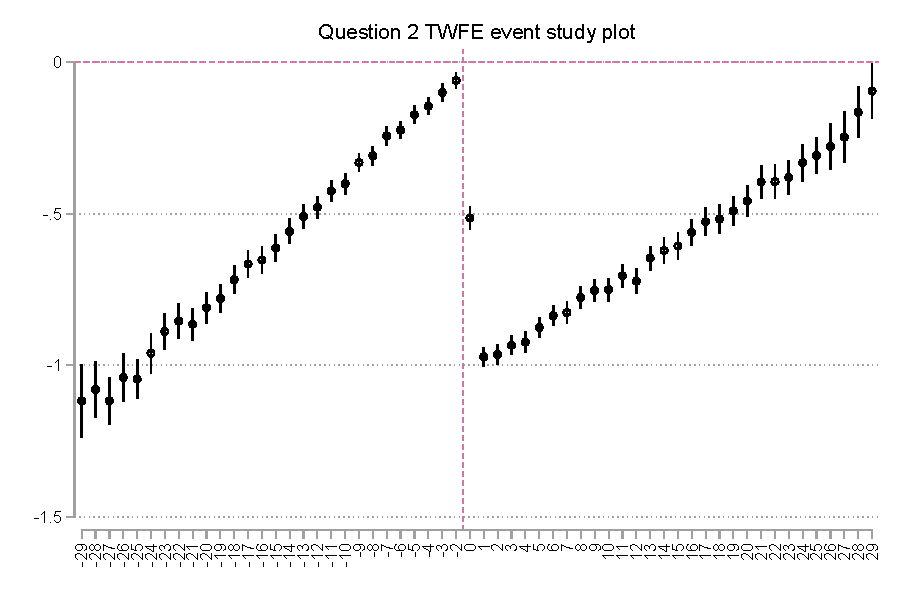
\includegraphics{hw6/question2plot.pdf}
    \caption{Event study plot for question 2}
    \label{fig:hw6q2}
\end{figure}

\begin{figure}
    \centering
    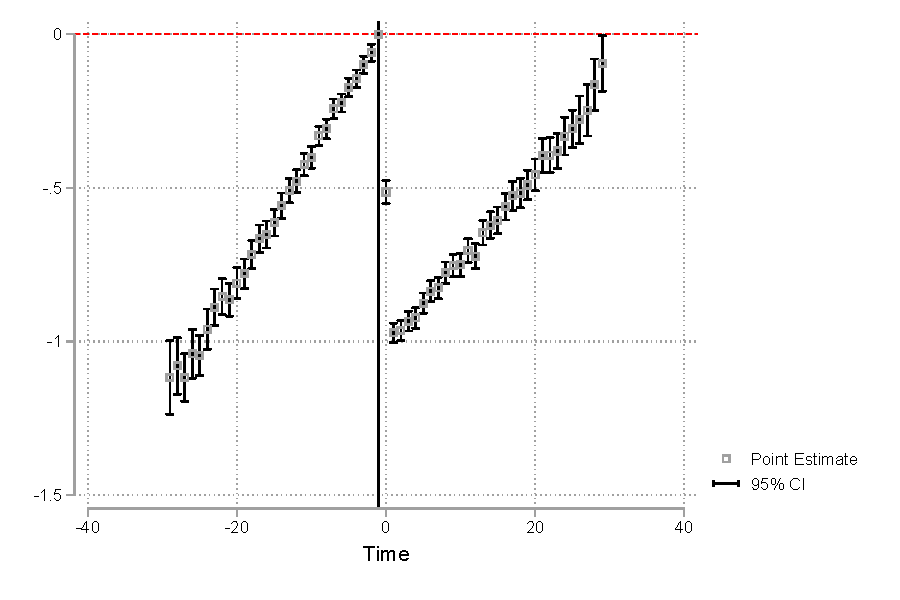
\includegraphics{hw6/question3plot.pdf}
    \caption{Event study plot for question 3}
    \label{fig:hw6q3}
\end{figure}

\begin{figure}
    \centering
    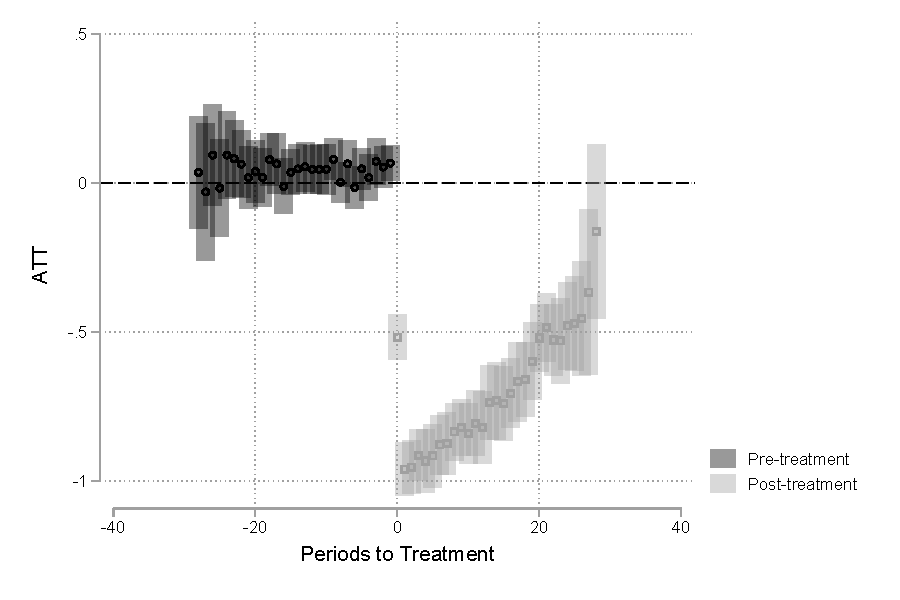
\includegraphics{hw6/question4plot.pdf}
    \caption{Event study plot for question 4}
    \label{fig:hw6q4}
\end{figure}
\end{document}

